
\begin{table}[h]
    \begin{subtable}[h]{0.45\textwidth}
    \begin{tabular}{|c|c|c|}
        \hline
        $m$ (massa) & $l$ (lunghezza) & $k$\\
        \hline

        $(19 \pm 1)\; g$  & $(108.0\pm 0.5) \;mm$ & $(70 \pm 20)\; Nm^{-1}$\\ 
        $(41 \pm 1)\; g$  & $(111.0 \pm 0.5) \;mm$ & $(73 \pm 9)\; Nm^{-1}$\\
        $(64 \pm 1)\; g$  & $(114.0 \pm 0.5) \;mm$ & $(74 \pm 6)\; Nm^{-1}$\\  
        $(74 \pm 1)\; g$  & $(115.5 \pm 0.5) \;mm$ & $(73 \pm 5)\; Nm^{-1}$\\ 
        $(91 \pm 1)\; g$  & $(118.5 \pm 0.5) \;mm$ & $(69 \pm 4)\; Nm^{-1}$\\ 
        $(95 \pm 1)\; g$  & $(119.5 \pm 0.5) \;mm$ & $(67 \pm 3)\; Nm^{-1}$\\ 
        $(134 \pm 1)\; g$  & $(127 \pm 0.5) \;mm$ & $(61 \pm 2)\; Nm^{-1}$\\ 


        \hline
    \end{tabular}
    \end{subtable}
    \hfill
    \begin{subtable}[h]{0.45\textwidth}
        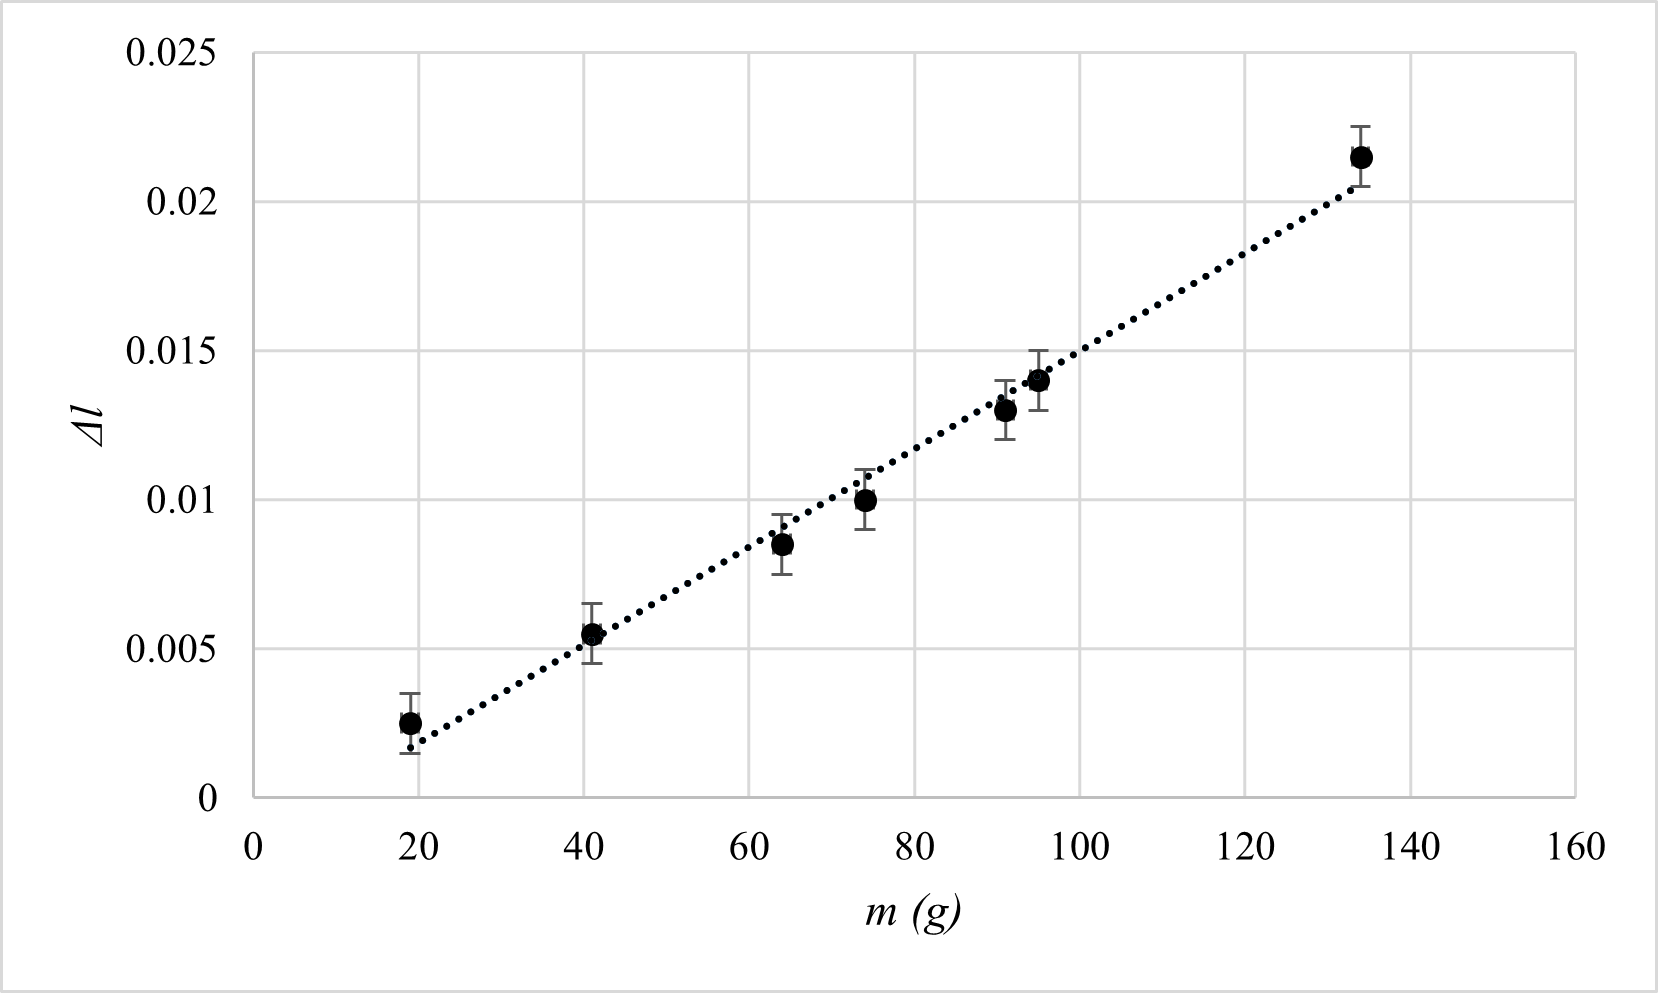
\includegraphics[width = 7cm]{plots/plt2mm.png}
    \end{subtable}
    \caption{Elastico $2\,mm$ ($l_0 = 105.5\, mm \pm 0.5\,mm$)$\qq \sigma_k = 5\; Nm^{-1}$}
    \label{tabellaElasitco2}
\end{table}
